\documentclass[class=scrartcl, crop=false]{standalone}

\usepackage[sexy]{/home/gautierk/.config/evan}
\usepackage{nicematrix}
\usetikzlibrary{shapes.geometric, calc}
\NiceMatrixOptions{transparent}

\title{Tutorial 6 - 10-11}

\begin{document}

\section{Tutorial 6: Permutation Groups}

% \subsection{Intuition about cosets}
% 
% $gH = \{gh : h \in H\}$

% \subsection{Back to permutation groups}

\begin{recall}
  
\begin{gather*}
  \begin{pmatrix}
    1 & 2 & 3 & 4 & 5 \\
    3 & 1 & 5 & 2 & 4
  \end{pmatrix}
  = (1 \ 3 \ 5 \ 4 \ 2)
\end{gather*}
\end{recall}

\begin{note}
  What is the order of a cycle $\sigma$ of length $r $?

  Answer: $|\sigma| = r$

  Reasoning: $\sigma = (x_0 \ x_1 \ \dots \ x_{r - 1})$

  $\sigma^m(x_i) = x_{i + m \ \text{(mod r)}}$ 

  So if $m = r$, $\sigma^m(x_i) = x_{i} \ \checkmark$
\end{note}

\begin{example}
  Show that $A_{10}$ contains an element of order 15.

  \begin{recall}
    $A_n$ = even permutations of $S_n$

    Every permutation $\sigma$ can be written as a product of transpositions.

    $(14356) = (16)(15)(13)(14)$. 

    There are an even number of transpositions. So  $(14356) \in A_n$
  \end{recall}

  \noindent
  First trying with $A_{15}$. $(1 \ 2 \ \dots \ 14 \ 15)$ is an example of an element with order 15. This is easy because we have access to 15 elements. \newline


  \noindent
  What about $A_{10}$?

  $\sigma = (1 \ 2 \ 3)(4 \ 5 \ 6 \ 7 \ 8)$

  $\sigma^m = ((1 \ 2 \ 3)(4 \ 5 \ 6 \ 7 \ 8))^m$

  \begin{note}
    $((1 \ 2)(3 \ 4))^2 = ((1 \ 2)(3 \ 4)(1 \ 2)(3 \ 4)) = (1 \ 2)^2(3 \ 4)^2$

    Only because the cycles are disjoint do they have this property.
  \end{note}

  \noindent
  Therefore $\sigma^m = ((1 \ 2 \ 3)(4 \ 5 \ 6 \ 7 \ 8))^m = (1 \ 2 \ 3)^m(4 \ 5 \ 6 \ 7 \ 8)^m$

  When does $(1 \ 2 \ 3)^m = (1)$? So long as  $3 \ | \ m$

  When does $(4 \ 5 \ 6 \ 7 \ 8)^m = (1)?$ So long as $5 \ | \ m$

  Therefore  $\sigma^m = (1) \Leftrightarrow \ 5 \ | \ m \ \ \text{and} \  \ 3 \ | \ m$

  Smallest such m is $m = 15$. Therefore $|\sigma| = 15$.

  $\sigma = (1 \ 3)(1 \ 2)(4 \ 8)(4 \ 7)(4 \ 6)(4 \ 5)$
\end{example}

\begin{exercise}
  Find $(a_1 \ a_2 \ \dots \ a_n)^{-1}$

  \begin{answer}
     $(a_1 \ a_2 \ \dots \ a_n)^{-1}= (a_n \ a_{n - 1} \ \dots \ a_1)$
  \end{answer}
\end{exercise}

\begin{example}
  \begin{enumerate}
    \ii[]
    \ii
    $(1 \ 7 \ 5 \ 4 \ 3)^{-1} = (3 4 5 7 1)$
    \ii
    $[(1 \ 4 \ 2 \ 3)(5 \ 6)(1 \ 3 \ 2)]^{-1} = (1 \ 3 \ 2)^{-1} \cdot (5 \ 6)^{-1} \cdot (1 \ 4 \ 2 \ 3)^{-1}$
    \ii
    $(1 \ 3 \ 5 \ 4 \ 7)^{702} = (1 \ 3 \ 5 \ 4 \ 7)^{700} \cdot (1 \ 3 \ 5 \ 4 \ 7)^{2} = (1) \cdot (1 \ 3 \ 5 \ 4 \ 7)^{2} = (1 \ 5 \ 7 \ 3 \ 4)$
  \end{enumerate}
\end{example}

\begin{exercise}
  $t = (a_1 \ a_2 \ \cdots \ a_k)$ is a cycle of length k

  \begin{enumerate}
    \ii
    Show that for any permutation $\sigma$, $\sigma t \sigma^{-1} = (\sigma(a_1) \ \sigma(a_2) \ \cdots \ \sigma(a_k))$

    This is equivalent to showing that 
    $\sigma t= (\sigma(a_1) \ \sigma(a_2) \ \cdots \ \sigma(a_k)) \sigma$
    \begin{enumerate}
      \ii
      Case where $x \notin \{a_1, \cdots, a_k\}$

      $\sigma t(x) = \sigma(x)$ because $t$ fixes x

      On the other hand, $(\sigma(a_1) \ \sigma(a_2) \ \cdots \ \sigma(a_k)) \sigma(x) = \sigma(x)$ because $\sigma(x) \neq \sigma(a_i)$ for all i.

      $\sigma(x) = \sigma(x) \ \checkmark$

      \ii
      Case where $x = a_i$ for some i.

      If  $i \neq k$, 

      $\sigma t(a_i) = \sigma(a_{i + 1})$

      $(\sigma(a_1) \ \sigma(a_2) \ \cdots \ \sigma(a_k)) \sigma(a_i) = \sigma(a_{i + 1})$ \newline

      If $i = k$,

      $\sigma t(a_k) = \sigma(a_1)$

      $(\sigma(a_1) \ \sigma(a_2) \ \cdots \ \sigma(a_k)) \sigma(a_k) = \sigma(a_1)$

    \end{enumerate}

    \ii
    Let $\mu$ be a cycle of length k.

    $t = (a_1 \ a_2 \ \cdots \ a_k)$

    Show that $\exists \sigma \in S_n$ such that $\sigma t \sigma^{-1} = \mu$ 

    We just showed that $\sigma t \sigma^{-1} = (\sigma(a_1) \ \sigma(a_{2}, \cdots \sigma(a_k))$

    Assume that $\mu = (b_1 \ b_2 \ \cdots \ b_k)$

    Let $\sigma$ be such that $\sigma(a_i) = b_i$ and $\sigma(x) = x$ if $x \neq a_i$ for all i, then the result follows.
  \end{enumerate}
\end{exercise}

\begin{exercise}
  Let there be group $G$ and fix $g \in G$.  Define $\lambda_g:G \to G$ where $\lambda(a) = ga$. Show that  $\lambda_g$ is a permutation.

  \begin{definition}
    A permutation of a set $S$ is a bijection $\pi : S \to S$
  \end{definition}

  \begin{enumerate}
    \ii
    Showing that $\lambda_g$ is injective.

    Let $a, b \in G$ such that $\lambda_g(a) = \lambda_g(b)$.

    $\Rightarrow ga = gb \Rightarrow a = b \ \checkmark$

    \ii
    Showing that $\lambda_g$ is surjective.

    For all $b \in G$, let $a = g^{-1}b \in G$. $\lambda_g(a) = gg^{-1}b = b$.

    Therefore the image of $\lambda_g$ is $G$ so $\lambda_g$ is surjective. $\checkmark$
  \end{enumerate}
\end{exercise}

\begin{exercise}[Dihedral Group]

  Using the cyclic notation, list the elements in $D_5$.

  $r = (1 \ 5 \ 4 \ 3 \ 2)$
  \quad
  $r^2 = (1 \ 4 \ 2 \ 5 \ 3)$
  \quad
  $r^3 = \dots$

  $s = (2 \ 5)(3 \ 4)$
  \quad
  $sr = \dots$
  
  \begin{center}
  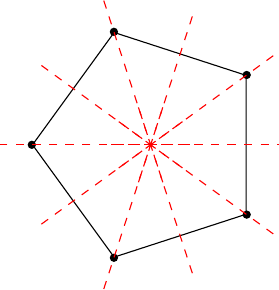
\begin{tikzpicture}[scale=3]
  \def\rps{5} % regular polygon sides
  \node (a) 
  [draw,  blue!0!black,rotate=90,minimum size=3cm,regular polygon, regular polygon sides=\rps] at (0, 0) {}; 

  \foreach \x in {1,2,...,\rps}
    \fill (a.corner \x) circle[radius=.5pt];
    \foreach \x in {1,2,...,\rps}{
    \draw [red,dashed, shorten <=-0.5cm,shorten >=-0.5cm](a.center) -- (a.side \x);
    \draw [red,dashed, shorten <=-0.5cm,shorten >=-0.5cm](a.center) -- (a.corner \x);}

  \end{tikzpicture}
  \end{center}
\end{exercise}

\begin{exercise}
  Show that $S_n$ is non-abelian for $n \geq 3$. We need to find $\sigma, \tau \in S_n$ such that $\sigma \tau \neq \tau \sigma$

  $\sigma = (1 \ 2)$
  \quad
  $\sigma = (1 \ 3)$ 

  $\sigma\tau = (1 \ 3 \ 2)$
  \quad
  $\tau\sigma= (1 \ 2 \ 3)$

  $(1 \ 3 \ 2) \neq (1 \ 2 \ 3)$

\end{exercise}

\end{document}
